\documentclass[12pt]{article} % use larger type; default would be 10pt
\usepackage[utf8]{inputenc} % set input encoding (not needed with XeLaTeX)

%%% PAGE DIMENSIONS
\usepackage{geometry} % to change the page dimensions
\geometry{a4paper} % or letterpaper (US) or a5paper or....
\geometry{margin=2cm} % or letterpaper (US) or a5paper or....

\usepackage{graphicx} % support the \includegraphics command and options
\usepackage[parfill]{parskip} % Activate to begin paragraphs with an empty line rather than an indent
\usepackage{times} % for Times Roman default font

%%% PACKAGES
\usepackage{booktabs} % for much better looking tables
\usepackage{array} % for better arrays (eg matrices) in maths
\usepackage{paralist} % very flexible & customisable lists (eg. enumerate/itemize, etc.)
\usepackage{verbatim} % adds environment for commenting out blocks of text & for better verbatim
\usepackage{subfig} % make it possible to include more than one captioned figure/table in a single float
\usepackage{caption}

%%% HEADERS & FOOTERS
\usepackage{fancyhdr} % This should be set AFTER setting up the page geometry
\pagestyle{fancy} % options: empty , plain , fancy
\renewcommand{\headrulewidth}{0pt} % customise the layout...
\lhead{}\chead{}\rhead{}
\lfoot{}\cfoot{\thepage}\rfoot{}

\makeatletter
\renewcommand{\maketitle}{%
  {\bfseries{\scshape{\Large{\@title\par}}}}
}
\makeatother

\hyphenation{Kiwi-bank} % otherwise it may get hyphenated as Ki-wibank

%%% END Article customizations

%%% The "real" document content comes below...

\title{Lake Man Biv Report: 3 September 2017}

\begin{document}
  \maketitle

\section{Background}

DoC have sought community support to maintain a number of huts/bivs in the Lewis Pass area, including Lucretia Biv and Lake Man Biv.  We have already expressed a willingness to help with the Lucretia Biv.  This document reports on a visit to Lake Man Biv on 3 September 2017.  The purpose of the visit was to assess the state of the Biv and determine whether or not we would be interested/capable of taking on its maintenance.

\section{Current state}

Lake Man Biv is a basic two-bunk biv, similar to Lucretia Biv but without a fire place.  The canvas of the bunks is in good condition and should last a few more years at least.

The Biv is basically sound, being in a similar condition to Lucretia Biv and better than Doubtful Hut (Figure \ref{DoubtfulHut}).  In particular, its sub-floor seems in good condition and, although there are signs of some water leakage in the past, it appears to be weather-proof now (Figure \ref{LMB1}).

\begin{figure}[ht]
%\centering
\begin{minipage}{.5\linewidth}
\begin{flushleft}
  \includegraphics[width=8cm]{LakeManBivRecce2Sep2017Photo1}
  \caption{Doubtful Hut}
  \label{DoubtfulHut}
\end{flushleft}
\end{minipage}
\begin{minipage}{.5\linewidth}
\begin{center}
  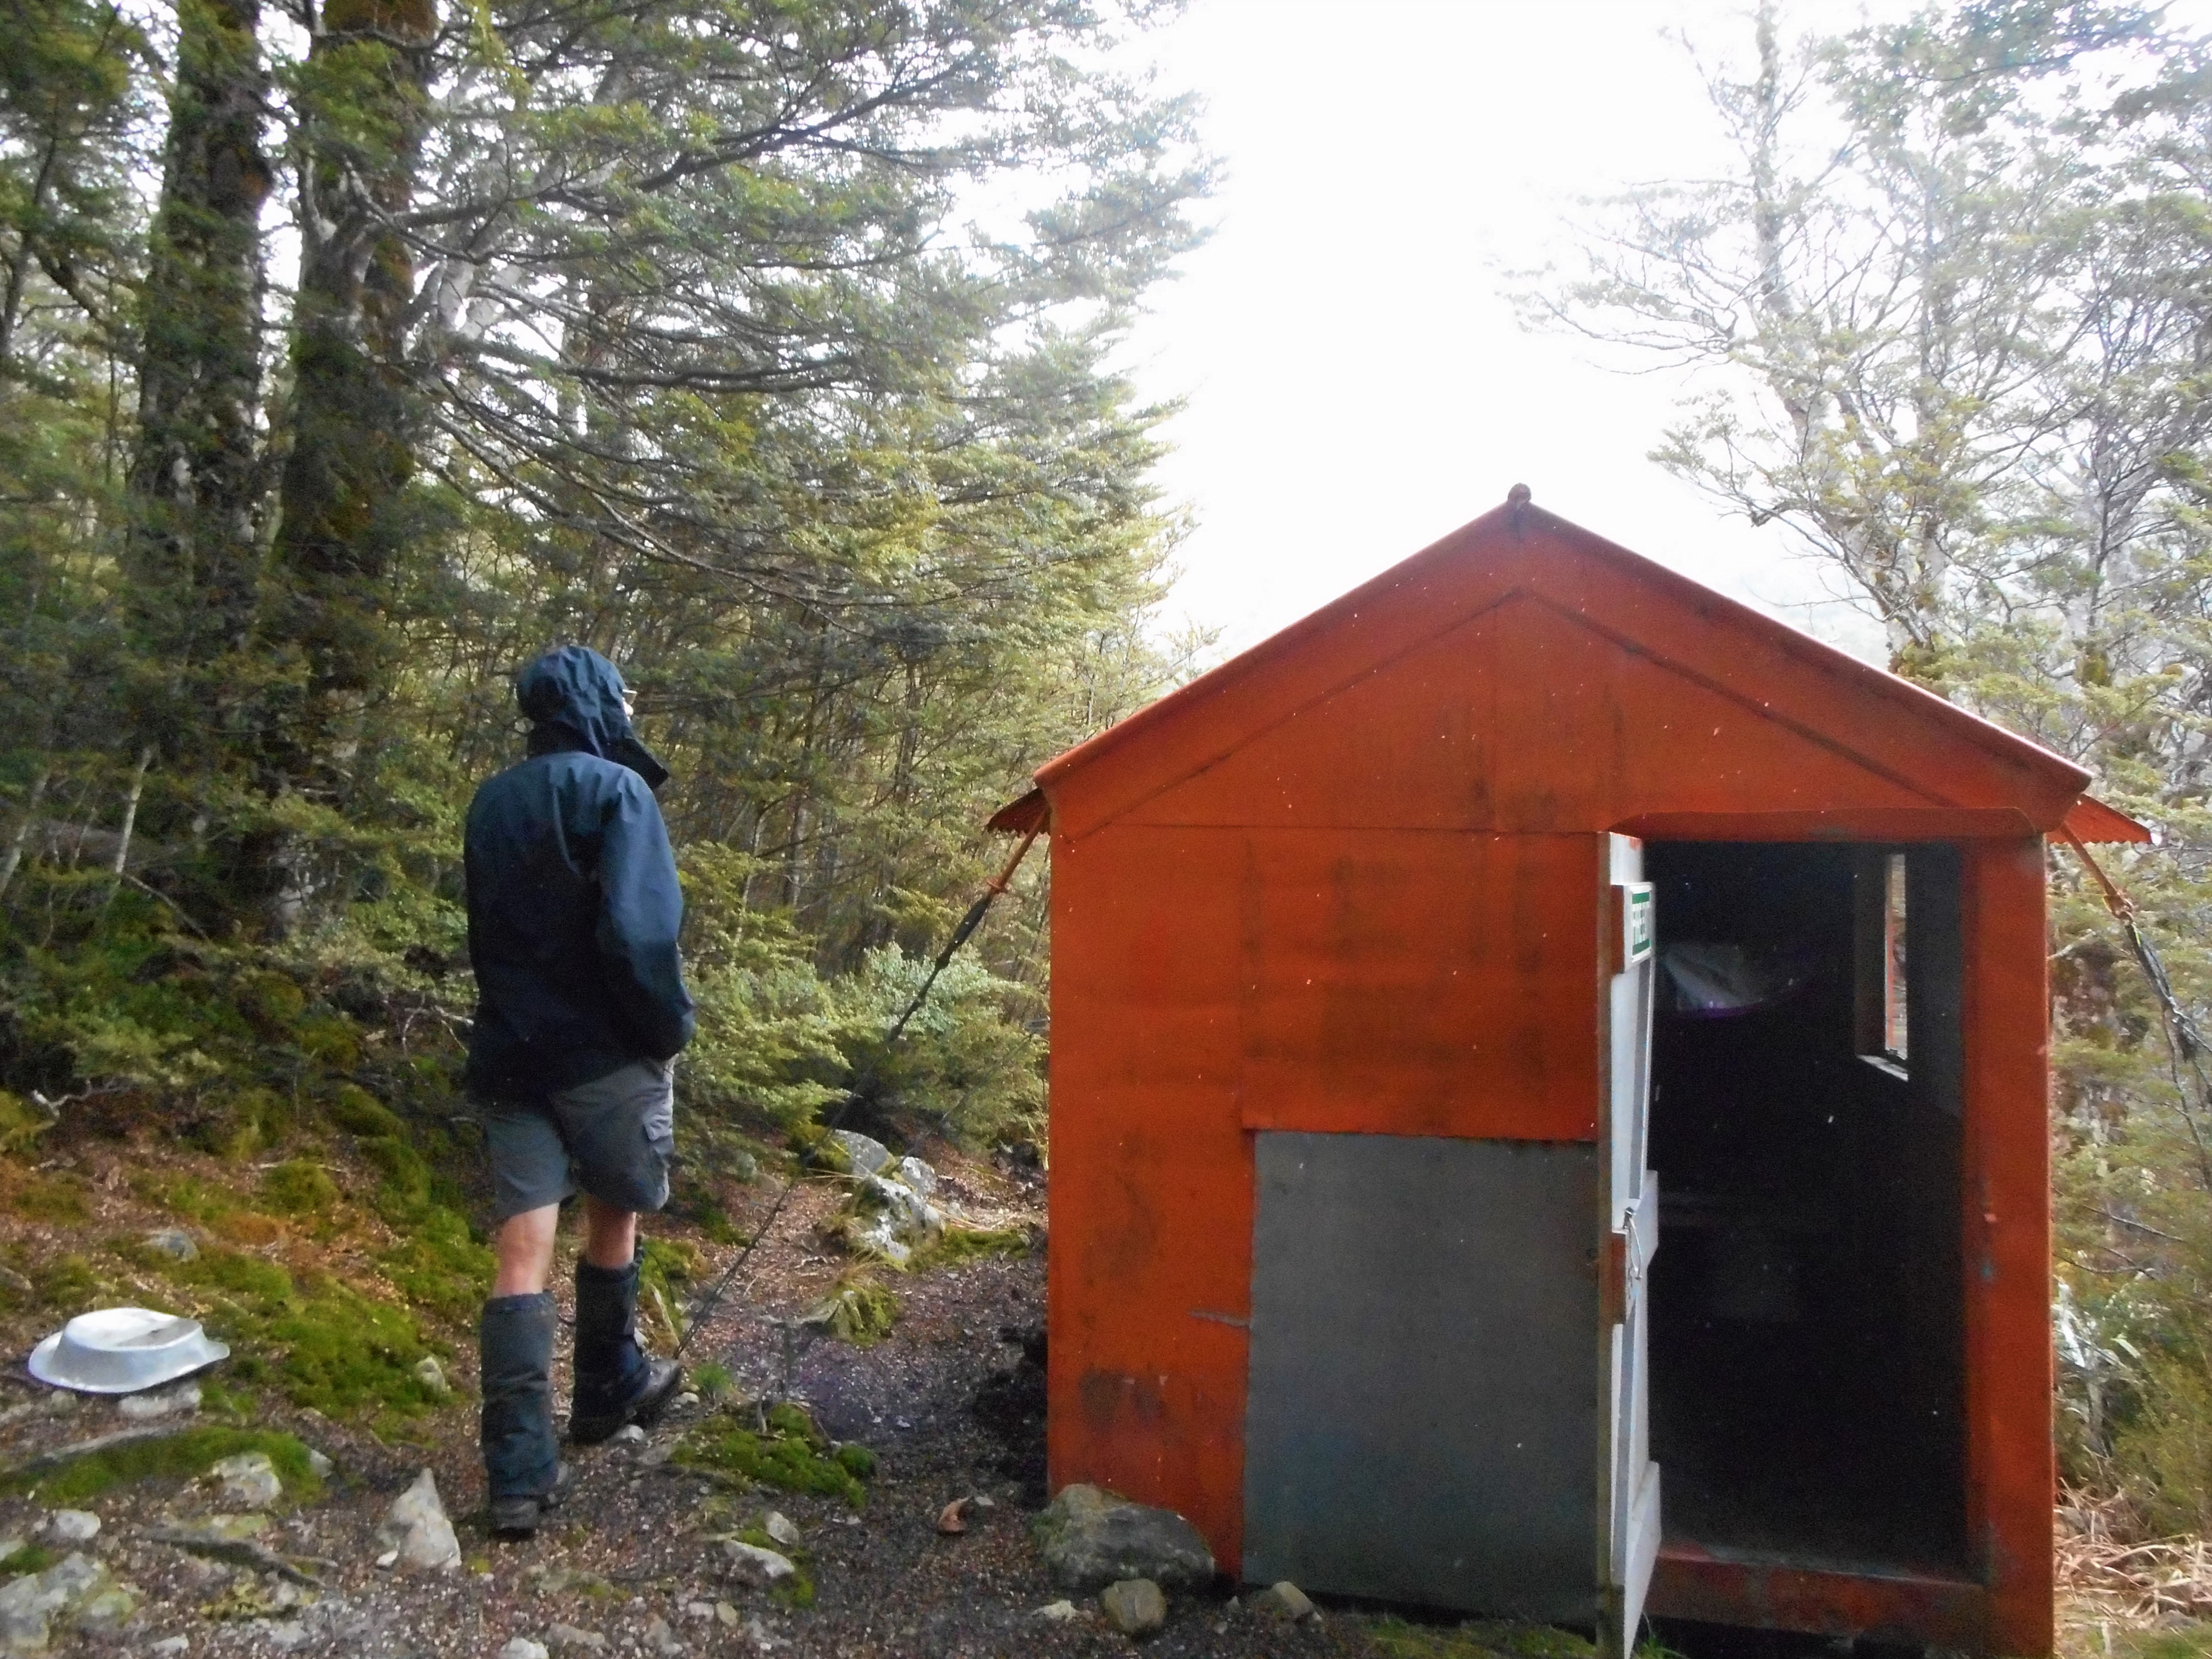
\includegraphics[width=8cm]{LakeManBivRecce2Sep2017Photo2}
  \caption{Lake Man Biv from the north.  Note the external patch behind which there is indication of internal water leakage in the past}
  \label{LMB1}
\end{center}
\end{minipage}
\end{figure}

\section{Maintenance and improvements}

\subsection{Required}

\begin{itemize}
 \item Replace the lead-head nails with hex-screws (there are about 90).  We didn't notice any sign of kea scratching the lead head nails, but replacement is a good precaution
 \item Paint the exterior.  This will involve quite a bit of preparation as the paint is in a sorry state, especially on the roof (Figure \ref{LMB2}).  An undercoat and two top coats would be required.  No rust was noted during the visit, but it is a good precaution to take a small pot of rust primer just in case
 \item Prior to painting there are a few small nail holes in the cladding which will need filling
 \item Dig a trench on the upper side of the biv to prevent leaf-litter building up on the lower cladding of the east wall (Figure \ref{LMB2}).  There is good elevation on the west side (Figure \ref{LMB3}), and thus such a trench would facilitate air movement under the floor
 \item Fit a weather ledge on the door to prevent water creeping under it during driving rain
 \item Remove some accumulated rubbish (about two rubbish bags)
 \item Since there is no long-drop, a suitable digging implement should be supplied.
\end{itemize}
 
\begin{figure}[ht]
%\centering
\begin{minipage}{.5\linewidth}
\begin{flushleft}
   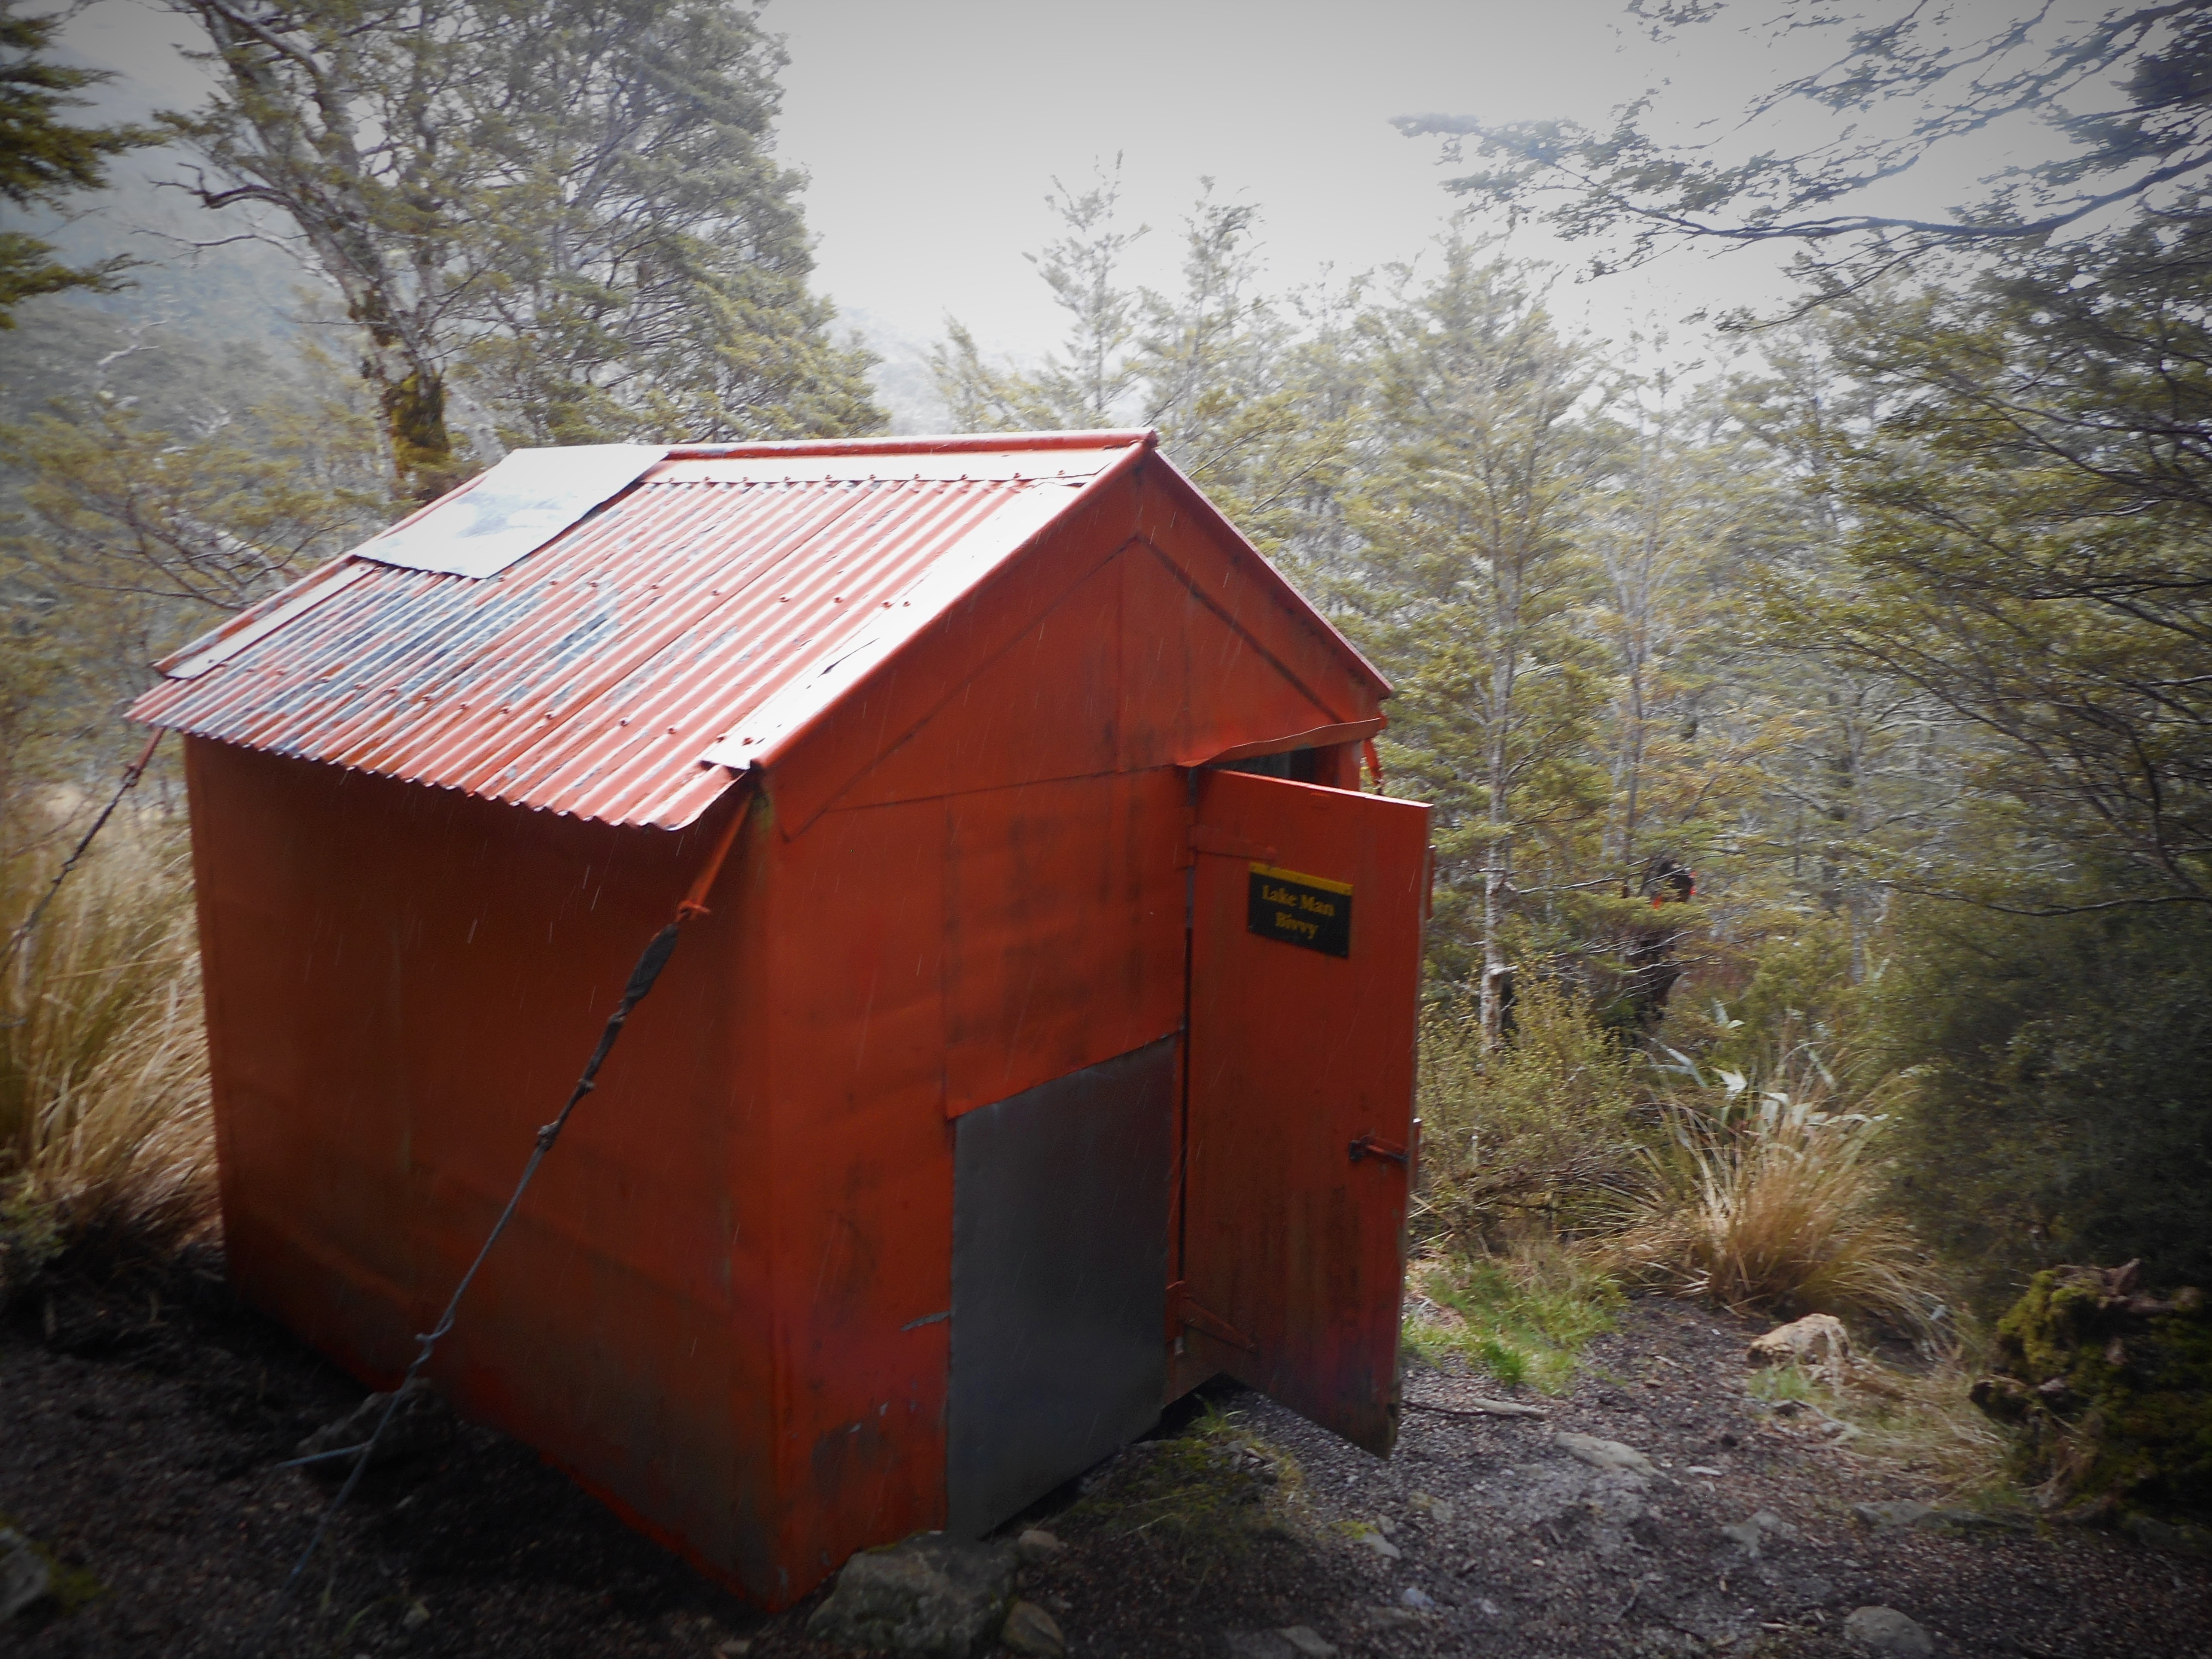
\includegraphics[width=8cm]{LakeManBivRecce2Sep2017Photo5}
   \caption{Lake Man Biv from the east}
   \label{LMB2}
\end{flushleft}
\end{minipage}
\begin{minipage}{.5\linewidth}
\begin{center}
   \includegraphics[width=8cm]{LakeManBivRecce2Sep2017Photo6}
   \caption{Lake Man Biv from the west}
   \label{LMB3}
\end{center}
\end{minipage}
\end{figure}

\subsection{Desirable}

\begin{itemize}
 \item As mentioned, the lead-head nails need replacing.  Thus, one might as well remove the roof and purlins, and install a ceiling lining (plywood painted white) and some insulation
 \item Internal trim around the doorway to reduce unwanted draft
 \item Better method of securing the door from the inside (i.e., an internal door bolt)
 \item Move (or replace) the bench, which is currently on the north wall to the east of the doorway (Figure \ref{LMB4}), to under the window.  This would have several advantages
 \begin{itemize}
   \item Allow the window to be more effective when providing ventilation during cooking
   \item Give better light on the cooking area
   \item Provide room for a mattress to be laid on the floor for a third person
 \end{itemize}
 \item Rebuild the shelves (Figure \ref{LMB4})
 \item Supply an extra mattress
 \item Install a small double-glazed window in the apex on the south wall (Figure \ref{LMB5}).  This would provide extra light and a nice view toward Mt Lakeman.  The existing window opens for ventilation, so this window need not do so.
\end{itemize}

\begin{figure}[ht]
%\centering
\begin{minipage}{.5\linewidth}
\begin{flushleft}
   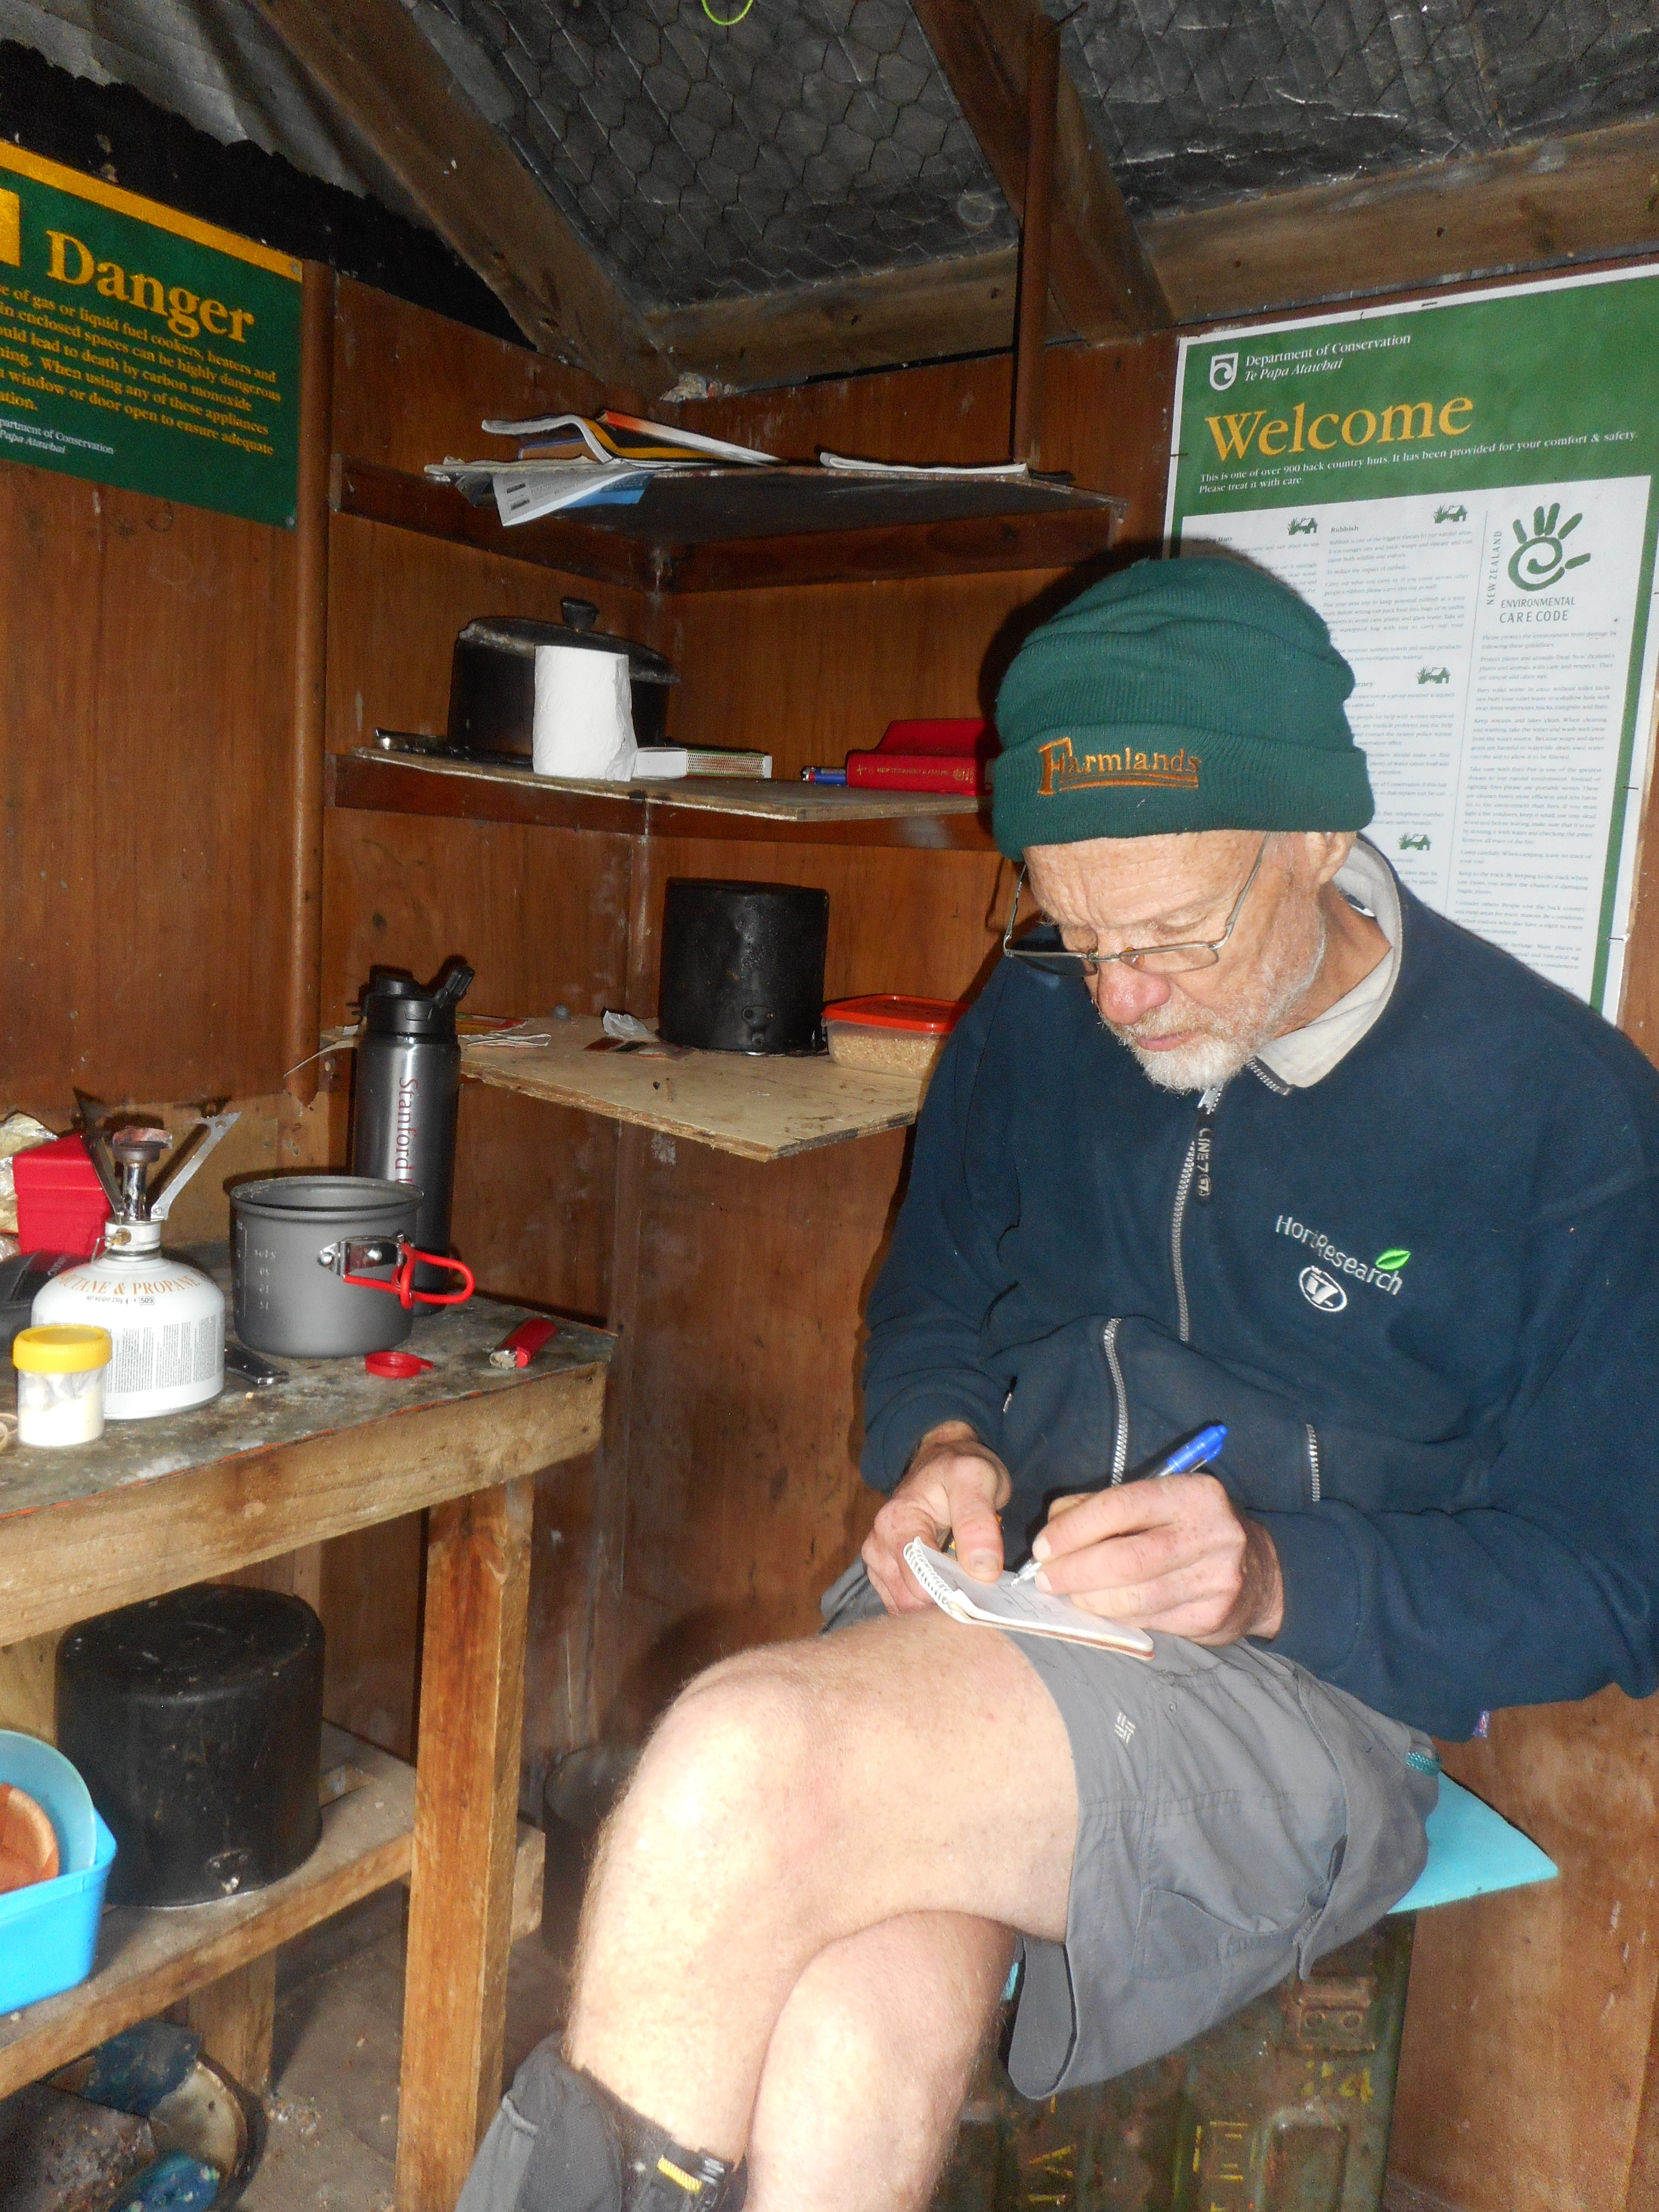
\includegraphics[width=8cm]{LakeManBivRecce2Sep2017Photo7}
   \caption{Lake Man Biv bench and shelves}
   \label{LMB4}
\end{flushleft}
\end{minipage}
\begin{minipage}{.5\linewidth}
\begin{center}
   \includegraphics[width=8cm]{LakeManBivRecce2Sep2017Photo8}
   \caption{Lake Man Biv from the south}
   \label{LMB5}
\end{center}
\end{minipage}
\end{figure}

\section{Estimated cost of materials}

\begin{table}[ht]
\caption{Estimated cost of materials.  NA means that the material will be donated (in the case of paint, by the DoC/Dulux Partnership Program), and ? means unknown} % title of Table
\label{costs}
\centering % used for centering table
\begin{tabular}{rr}
\hline
Material & Cost est. \\ [0.5ex]
\hline % inserts single horizontal line
Box of 100 65mm hex-screws & \$50.00\\
Mould/lichen cleaner & NA\\
Rust primer & NA\\
Exterior undercoat (1 litre) & NA\\
Exterior top coat (4 litres) & NA\\
Brushes etc & NA\\
Two sheets of 9mm ply & \$70.00 \\
Insulation & ?\\
Undercoat for ply & NA \\
1 litre top coat for ply & NA \\
Tube of silicon & \$15.00 \\
Internal bolt & \$5.00 \\
Timber for bench and shelving & \$100.00 \\
Bench top (second-hand stainless steel) & ?\\
Extra mattress & ?\\
Window & \$350.00 \\
Pick-axe for digging toilet holes & NA \\
Contingencies (10\%) & \\ [1ex] % [1ex] adds vertical space
\hline \\
TOTAL & \\
\hline \hline %inserts single line
\end{tabular}
\label{costs} % is used to refer this table in the text
\end{table}

The costings provided in Table \ref{costs} are only approximations.  Notes:

\begin{itemize}
 \item The total exterior surface area for painting is approximately 20m$^2$
 \item Since only a small amount of insulation would be required it is likely this can be obtained for a small cost via TradeMe or similar
 \item If the existing bench is simply moved then there is no cost.  However, it might be possible to get a second-hand stainless version at little cost
\end{itemize}

Thus the total cost of the materials will be less than \$1000.  There are also chopper costs to ferry the materials and tools in, and tools and rubbish out (approximately \$3000 for the two trips).  Given that we are (mostly) retired and thus flexible as to when the job is done, it may be possible to arrange this as part of a larger operation in the area.  Labour, of course, will be voluntary.

\begin{flushright}
Peter Alspach \& Robyn Ritchie\\
paalspach@gmail.com
\end{flushright}

\end{document}
